\documentclass[11pt]{article}
\usepackage{multicol}
% \usepackage{fullpage}
\usepackage{url}
\usepackage{graphicx}
\usepackage[small]{titlesec}
\begin{document}
\title      {\textbf{COMP6026: Assignment 2}}
\author	    {Thomas Smith\\taes1g09@ecs.soton.ac.uk}
\date       {\today}
\maketitle
% \begin{multicols}{2}
\section{Introduction}
1.5 pages
% o   Introduction: You need not spend more than 1.5 pages describing the original paper.
% ?         briefly describe the paper/experiment
% ?         What you evolved including
% ?         How you represented individuals
% ?         What fitness function did you define
% ?         What kind of GA you used
% ?         Steady state/ generational?  Tournament selection/ fitness proportionate (roulette wheel)?
% ?         What kind of crossover (if any) you used.
% ?         All parameters (enough detail so a reader could re-implement the GA)

%basic introduction
In this paper we reimplement the resulst of [Watson 2009] TODO , and show that [their conclusion holds]. We ther present the results of further analysis, which show that [my hypothesis is proven correct].
\section{Reimplementation}
%description of original paper

\subsection{Representation}
For an efficient and quick algorithm, correct representation is important
First we did this
then we did this
Allowed quick computation, horray

\subsection{Parameters}
We used the parameters as in the original palper, plus these
[table]
Parameter
Value
Growth rate (cooperative), Gc
0.018
Growth rate (selfish), Gs
0.02
Consumption rate (cooperative), Cc
0.1
Consumption rate (selfish), Cs
0.2
Population size, N
4000
Number of generations, T
1000

% var GROUP_SIZE = [40, 4];
% 			var DEATH_RATE = 0.1;
% 			var INFLUX_RATE = [50, 4];
% 			//from section 3 of paper [coop, self]
% 			var GROWTH_R = [0.018, 0.02];
% 			var CONSUME_R = [0.1, 0.2];
% 			var N = 4000;
% 			var T = 120;
% 			var t = 4;

\begin{table}[!htb]
  \centering
  \begin{tabular}{r|c|ccr|c}
  Behaviour parameters	& Cooperative	& Selfish	&  & \multicolumn{1}{c}{} & \\ \cline{1-3}
  Growth rate 			& 0.018			& 0.02		&  & Global parameters	& Value\\ \cline{5-6}
  Consumption rate 		& 0.1			& 0.2		&  & Population size, $N$	& 4000\\
  \multicolumn{1}{r}{} & \multicolumn{1}{c}{} & \multicolumn{1}{c}{} &  & Generations, $T$ & 120 \\
  Size parameters		& Large			& Small		&  & Reproduction cycles, $t$~ 		& 4\\ \cline{1-3}
  Group size			& 40			& 4			&  & Death rate, $K$ & 0.1\\
  Resource influx		& 50			& 4			&  & \multicolumn{1}{c}{} & \\
  \end{tabular}
  \caption{Parameters from \cite{orig}, used throughout the reimplementation.}
  \label{Table:table1}
\end{table}

\subsection{Results}
~1 page
% o   Reimplementated Results (~1 page)
% ?         The reimplemented figures (side by side with the originals)
% ?         Discussion of what the results show/don't show, what worked/didn't work, what you learned
\begin{figure}[!ht]
  \centering
  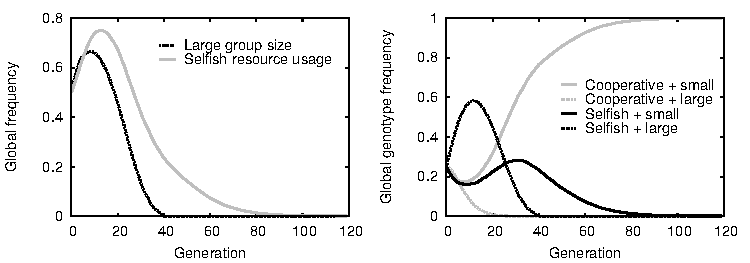
\includegraphics{plot.pdf}
  \caption{My plot.}
  \label{Figure:plot}
\end{figure}

\begin{figure}[!ht]
  \centering
  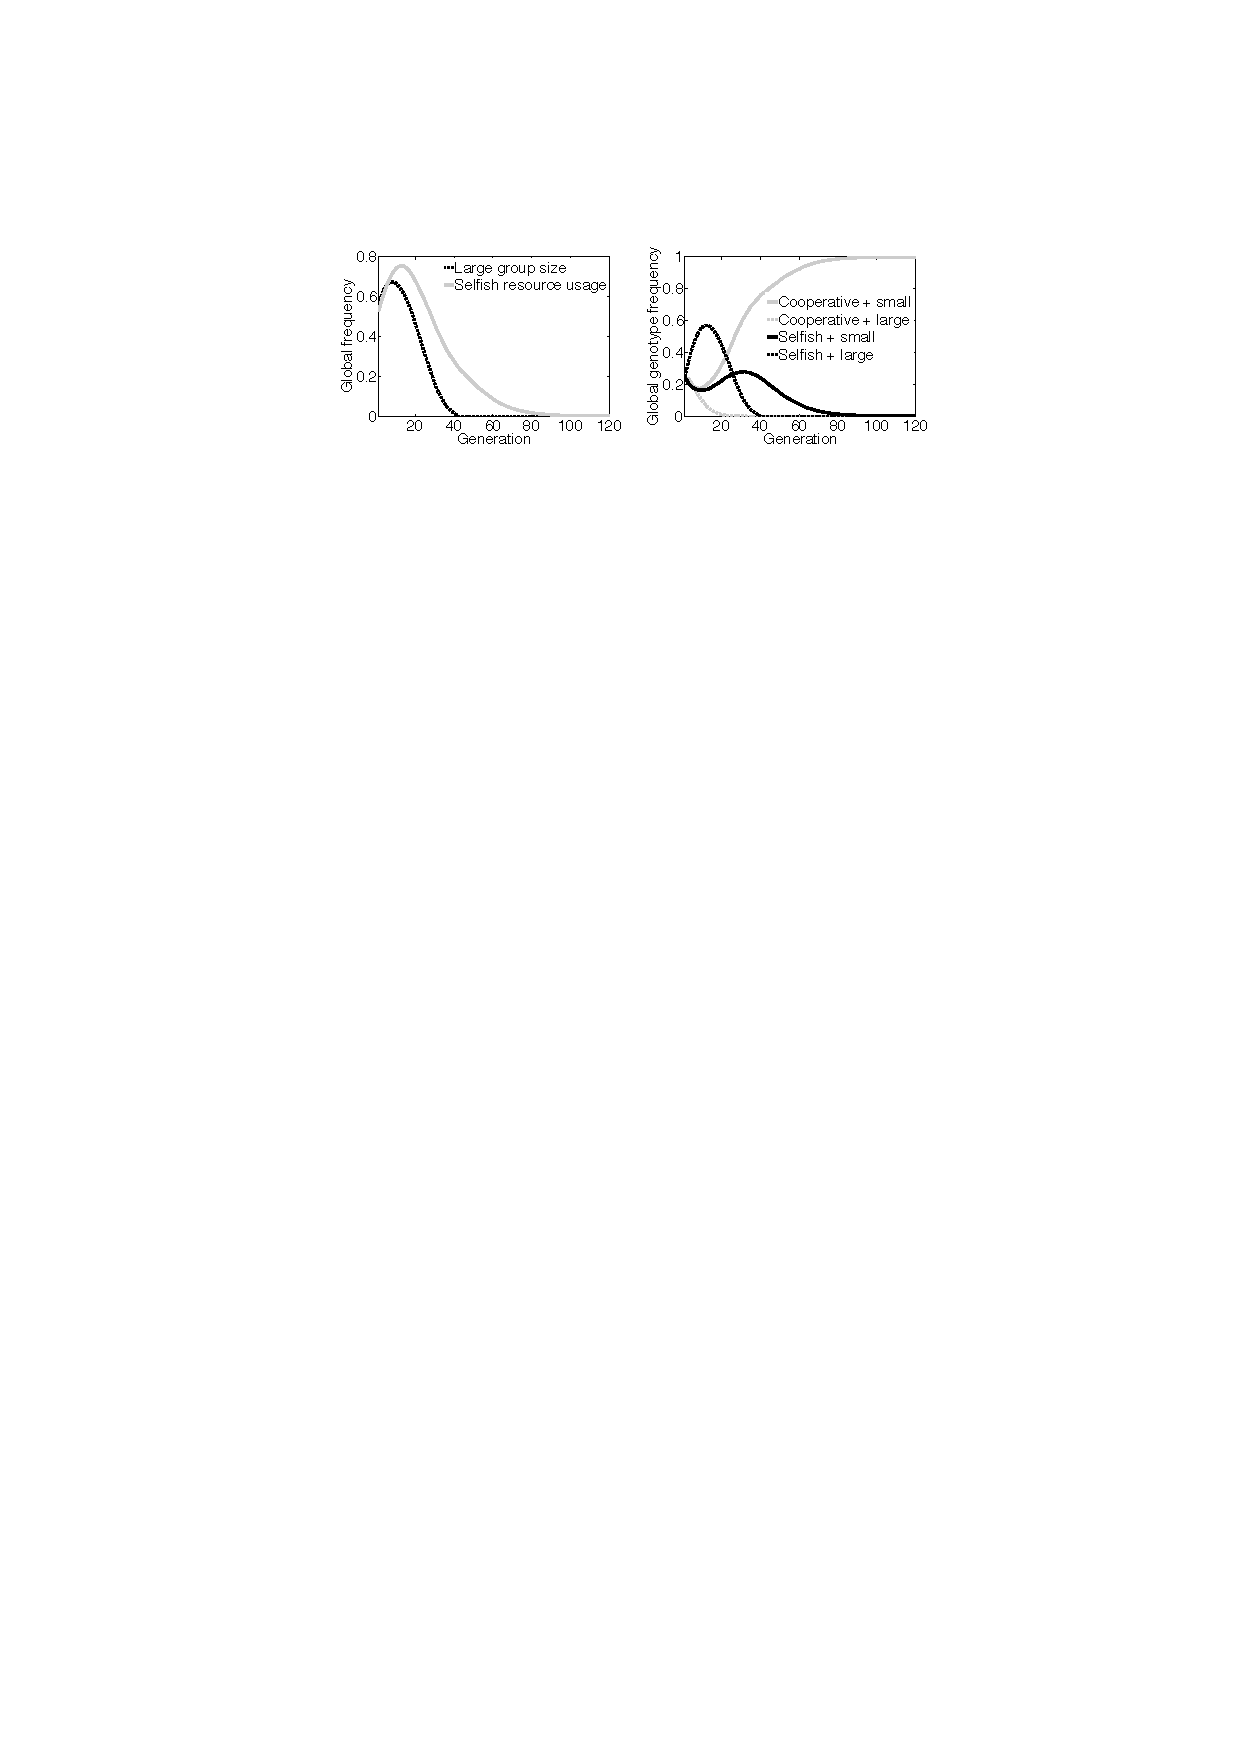
\includegraphics[scale=1.25]{original.pdf}
  \caption{original plot.}
  \label{Figure:original}
\end{figure}

\section{Extension}
~1 page
% o   Describe your extension  (another page)
% ?        What is your research question/hypothesis?
% ?         e.g., 'compare x with y' or 'add x and see what difference it makes compared to not(x)'.
% ?         Describe methods
% ?         Any advancements you made
% ?         Support the value of asking that question (using literature)
% ?         What do you expect to happen (what might happen)?
% ?         Why do you think that?

\subsection{Representation}
\subsection{Results}
~1.5 pages
% o   Results of extension (another 1.5 page)

\section{Conclusion}
~1 page
% o  What do you conclude from that -- significance of the extension results/critique/evaluation (final page)

\section*{References}
\begin{thebibliography}{9}

\bibitem{orig} 
Powers, S., Penn, A., Watson, A.: Individual Selection for Cooperative Group Formation. Advances in Artificial Life: Proceedings of the Ninth European Conference on Artificial Life (ECAL 2007) (2007) 585--594

\end{thebibliography}

\appendix
\section{Source}
% Appendix: source code of what you implemented (include the source of everything you implemented as part of the pdf)
% You may also upload a zip of all source code (if this includes any code you did not implement -- it must be clearly declared in a README file, and at the front of the report)

% \end{multicols}
\end{document}


What to include in your assign 2 report
See separate marks scheme for marking details.
o   Introduction: You need not spend more than 1.5 pages describing the original paper.
?         briefly describe the paper/experiment
?         What you evolved including
?         How you represented individuals
?         What fitness function did you define
? What kind of GA you used
?         Steady state/ generational?  Tournament selection/ fitness proportionate (roulette wheel)?
?         What kind of crossover (if any) you used.
?         All parameters (enough detail so a reader could re-implement the GA)
o   Reimplementated Results (~1 page)
?         The reimplemented figures (side by side with the originals)
?         Discussion of what the results show/don't show, what worked/didn't work, what you learned
o   Describe your extension  (another page)
?        What is your research question/hypothesis?
?         e.g., 'compare x with y' or 'add x and see what difference it makes compared to not(x)'.
?         Describe methods
Any advancements you made
?         Support the value of asking that question (using literature)
What do you expect to happen (what might happen)?
Why do you think that?
o   Results of extension (another 1.5 page)
o  What do you conclude from that -- significance of the extension results/critique/evaluation (final page)
Appendix: source code of what you implemented (include the source of everything you implemented as part of the pdf)
You may also upload a zip of all source code (if this includes any code you did not implement -- it must be clearly declared in a README file, and at the front of the report)
 

 particular aggregation and dispersal metapopulation structure that we have modelled. 